%BeginFileInfo
%%Publisher=TEMP
%%Project=VYTAS
%%Manuscript=AICOM2E
%%Stage=100
%%TID=Vytas
%%Format=latex
%%Distribution=live
%%Destination=PDF
%%DVI.Maker=vtex_tex_dvi
%%PDF.Maker=live_tex_pdf
%%DVX.Maker=vtex_tex_dvx
%%Compiler cmd line=LATEX612.BAT %N.TEX
%EndFileInfo
% Journal: Applied Ontology, IOS Press
% Latex 2e
% Test file ao2e.tex
%
\documentclass{ao2e}%[seceqn,secfloat,secthm]
\usepackage[T1]{fontenc}
\usepackage{times}%
\usepackage{natbib}
\usepackage{moreverb}
\usepackage[nolist]{acronym}
\usepackage{url}
%\usepackage{pdftex} 
\usepackage{graphicx} 

\newcommand{\protege}{Prot\'{e}g\'{e}}
%\usepackage{todonotes}

%\firstpage{1}
%\lastpage{3}
%\volume{3}
\pubyear{2009}

\begin{document}
\begin{frontmatter}                           % The preamble begins here.
%
%\pretitle{Pretitle}
\title{ MIREOT: the Minimum Information to Reference an External Ontology Term}
\runningtitle{MIREOT: the Minimum Information to Reference an External Ontology Term}
%\subtitle{Subtitle}

\author[A]{\fnms{M\'elanie} \snm{Courtot}%
\thanks{Corresponding author: M\'elanie Courtot, BC Cancer Agency, Vancouver, BC, Canada.}},
\author[B]{\fnms{Frank} \snm{Gibson}},
\author[C]{\fnms{Allyson L.} \snm{Lister}},
\author[D]{\fnms{James} \snm{Malone}},
\author[E]{\fnms{Daniel} \snm{Schober}},
\author[A]{\fnms{Ryan R.} \snm{Brinkman}}
and
\author[F]{\fnms{Alan} \snm{Ruttenberg}}

\runningauthor{M. Courtot et al.}
\address[A]{BC Cancer Agency, Vancouver, BC, Canada\\
E-mail: mcourtot@gmail.com, rbrinkman@bccrc.ca}

\address[B]{Abcam plc, 332 Cambridge Science Park, Cambridge, CB4 OWN, UK\\
E-mail: fgibson@gmail.com}

\address[C]{CISBAN and School of Computing Science, Newcastle University, Newcastle upon Tyne, UK\\
E-mail: a.l.lister@newcastle.ac.uk}

\address[D]{The European Bioinformatics Institute, Cambridge, CB10 1SD, UK\\
E-mail: malone@ebi.ac.uk}

\address[E]{Institute of Medical Biometry and Medical Informatics (IMBI), University Medical Center, 70104 Freiburg, Germany\\
E-mail: schober@imbi.uni-freiburg.de}

\address[F]{Science Commons, Cambridge, MA, USA\\
E-mail: alanruttenberg@gmail.com}


\begin{abstract}
While the Web Ontology Language (OWL) provides a mechanism to import ontologies, this mechanism is not always suitable.
Current editing tools present challenges for working with large ontologies and direct OWL imports can prove impractical for day-to-day development.
Furthermore, external ontologies often undergo continuous change which can introduce conflicts when integrated with multiple efforts.
Finally, importing heterogeneous ontologies in their entirety may lead to inconsistencies or unintended inferences.
In this paper we propose a set of guidelines for importing required terms from an external resource into a target ontology.
We describe the methodology and a tool which implements the approach, present some examples of this application, and outline future work and extensions.
\end{abstract}


\begin{keyword}
ontology import\sep data integration\sep MIREOT
\end{keyword}

\end{frontmatter}

\section{Introduction}

The ability to share and reuse existing ontological resources is an important consideration when developing a new ontology.
For example, when developing an ontology related to the biomedical domain, it may be useful to include terms from the \ac{GO}\cite{GO} to represent biological processes or from \ac{PATO}\cite{PATO} to represent properties of entities.
Ontologies such as GO and PATO are built collaboratively by communities of experts and are the products of substantial effort.
Recapitulating this work instead of reusing it represents a duplication of development effort and results in duplicate ontologies covering the same domain. It could also result in projects having different unique identifiers to denote the same entity, which would require post-hoc, error prone, identifier mapping systems to enable data integration. 
While it appears that building upon existing vocabularies is the best way to proceed, ontology developers are faced with some difficulties when actually trying to do so.
The easiest way to integrate an existing body of work is to rely on the \ac{OWL} \cite{OWL} mechanism \emph{owl:imports}, which imports the external resource as a whole. However current limitations in tools and reasoners can sometimes make this impractical.
Popular OWL tools (\emph{e.g.}, Prot\'eg\'e, Pellet) can neither load nor reason %\todo{give example of reasoner?} MC: hard to add here, and those tools embed reasoners.
over very large ontologies such as the NCBI Taxonomy \cite{NCBI} or the Foundational Model of Anatomy \cite{FMA}, making direct \ac{OWL} imports of such important resources impractical. 
Furthermore, external ontologies may have been constructed using design principles which may not align with the practice of the ontology wishing to import them.  In this instance, importing such ontologies as a whole could lead to inconsistencies or unintended inferences. %\todo such as what? this is a bold statement - is it backed up anywhere else?
Other import options are possible, for instance using software that extracts a \emph{module} \cite{Grau} of the external ontology.
A module can be seen as a fragment of an external ontology that, when imported by an other ontology, allows the same inferences to be drawn with respect to the classes of interest as if the whole ontology had been imported. This solution allows developers to pick only pieces of the source ontology (and thus overcome size issues) without losing any reasoning power.
However, if an extracted module is to be useful, the external ontology needs to be structured in a way that is compatible with the importing ontology (for example, using the same upper ontology and relationship types), and the logical axioms need to be accurate. 
This is not always the case at the current stage of development of some ontologies.
For example, during the development of the \ac{OBI}\cite{OBI}, importing the root class of the \ac{CARO}\cite{CARO} was not desired as its definition intersected multiple classes in \ac{OBI} that was not considered useful. %\todo JM: I don't understand this sentence so I haven't reworded it - when you say not considered useful do you actually mean, more strongly, it was incorrect?

In addition, although software that extracts \emph{modules} are available, most are only in early stages of development.

We tried several modularization tools \cite{Grau2} \cite{Jimenez}  \cite{Seidenberg} \cite{Sirin}. 
All of them discarded annotations, resulting in modules containing only the class declarations, and no annotation properties, such as labels or definitions.
We also experienced software crashes on large ontologies (the size of the ontologies capable of being loaded varied with the tool, for example we were able to load ChEBI \cite{ChEBI} with SWOOP but not with Prot\'eg\'e 3.4).
One tool %RB:\todo{which?} %MC: Seidenberg - but the tools have no name, so it is difficult to refer to them.
had undocumented assumptions about the form of URIs used as class names and therefore extracted empty modules. 
Finally, tools %RB:\todo{which?}%MC: the others :)
that were able to extract modules either extracted a single term or a large number of them (depending on the arguments passed), as they try and approximate a module without discarding potentially useful information. These large modules undermine the goal of having imports of a manageable size.
Our conclusion is that the current ontology tool set is in the early stages of development and, though promising, each presents a trade-off. %\todo JM: I think saying "`none of them can be used whatsoever"' is too sweeping a statement and not backed up enough so i have removed this. it is enough i think to say they all have weaknesses.

To address these issues we developed a set of guidelines for importing terms from multiple ontology resources, avoiding the overhead of importing the complete ontology from which the terms derive. 

The \ac{MIREOT} guidelines were created to aid the development of the \ac{OBI}.
\ac{OBI} uses the \ac{BFO} \cite{BFO} as an upper-level ontology and has been submitted for inclusion in the \ac{OBO} Foundry \cite{OBOFoundry}. 
One of the fundamental principles of the \ac{OBO} Foundry is to reuse, where appropriate, existing ontology resources, therefore avoiding duplication of effort and ensuring orthogonality.
\ac{MIREOT} provides a mechniasm by which external ontology terms can be selectively imported, even if they do not use a particular upper ontology or even OWL DL.

\section{Policy}

In deciding upon a minimum unit of import, our first step was to consider the practice of other ontology efforts.
For example, in the \ac{GO}, the intended denotation of classes remains stable such that even when the ontology is repaired or reorganized, the effects of such changes do not affect the intended meaning of individual terms.
Rather, the changes are towards more carefully expressing the logical relations between them.
When a term's definition changes meaning, the term is deprecated \cite{GOGuide}.
We can therefore consider a term as stable, in isolation from the rest of the ontology, and use terms (i.e. individual classes in isolation from the ontology) as basic unit of import.
The current implementation of \ac{MIREOT} has been limited to import of terms from other ontologies that aspire to the OBO Foundry, and so adhere to a similar deprecation policy.

The minimum amount of information needed to reference an external class is the source ontology URI (\textit {i.e.}, where the term comes from) and the external term's URI (\textit {i.e.}, the identifier for this term). 
Generally, these items remain stable and can be used to unambiguously reference the external class from within the importing target ontology.
The minimum amount of information to integrate this class is its desired position in the hierarchy, specifically the URI of its direct superclass in the target ontology (\textit {i.e.}, under which class the term is asserted)

Taken together, the following minimal set is enough to consistently reference an external term:
\begin{itemize}
 \item \textbf{source ontology URI} The logical URI of the ontology containing the external term to be imported. 
 \item \textbf{source term URI} The logical URI of the specific term to import. 
 \item \textbf{target direct superclass URI} The logical URI of the direct asserted superclass in the importing ontology.
\end{itemize} 

To ease development of the importing ontology we also recommend, although do not require, that additional information about the external class be added, such as its label and textual definition, or any other kind of information that may be deemed useful by the ontology developers.
This additional information, when appropriate, is mapped into the importing ontology's annotation properties.

To keep this information current, the imports are stored in a separate file that can be removed and rebuilt on a regular basis. This introduces an additional level of modularity, separating the domain ontology of interest with the external ontologies.


\section{Implementation}

An implementation of the \ac{MIREOT} guidelines was performed in the context of the \ac{OBI} project, and can be decomposed into a two-step process:

\begin{enumerate}
\item Gather the minimum information for the external class.
\item Use this minimum information to fetch additional elements, like labels and definitions.
\end{enumerate}

Once the external term is identified for import, the first step is to gather the corresponding minimum information set.

This set is stored in a file called \emph{external.owl}. (All scripts and files are available under the \ac{OBI} Subversion Repository \cite{OBIScripts}).
In the current implementation, a Perl script, \emph{add-to-external.pl}, can be used to append the minimum information set to the \emph{external.owl} file, or the information can be entered in an ontology editing tool. In the future we anticipate this operation will have specific support within editing tools.

The script takes as arguments the identifier of the external class to be imported and its parent class in the target hierarchy.
In addition, a mapping between the prefix used in the identifier and the external source ontology URI is built into the script.
Curators therefore need only specify the ID of the external class to import and the ID of the class it should be imported under.

In the current implementation, additional elements can be obtained programmatically via SPARQL\cite{SPARQL} CONSTRUCT queries, as described in Figure \ref{fig:sparql}.
These queries\cite{OBIQueries} specify, for each source ontology, which extra information about the class to gather, such as the definition and preferred label, and how to map these into the corresponding OBI annotation properties. However as module extraction technology matures, and where appropriate, additional elements could be retrieved using such technology.

\begin{figure}[t]
\scriptsize
\verbatiminput{./figs/sparql.txt} 
\caption{Template SPARQL query. For convenience, we use alias:preferredTerm and
alias:definition to reference our annotations properties IAO\_0000111 and IAO\_0000115 \cite{IAO} respectively. The \_ID\_GOES\_HERE\_ pattern will be replaced by the script when building the CONSTRUCT query.}
\label{fig:sparql}
\end{figure}

For example, in the current \ac{OWL} rendering of \ac{OBO} files, definitions are individuals and the rdfs:label of those individuals record the text of the definitions. 

Within the \ac{OBI} implementation of the \ac{MIREOT} guidelines, the value of the rdfs:label of the oboInOwl:Definition will be set to the value of iao:definition. Only annotation properties which map directly to the target ontology's own metadata are copied; new properties, if not specified in the source ontology, are not created. The external term's property values are copied \emph{"as-is"} from the external resource.

Finally, a script, \emph{create-external-derived.lisp}, iterates through the minimum information stored in \emph{external.owl}.
Depending on the source ontology URI of each of our imported terms, it then selects the correct SPARQL template and substitutes the relevant ID.
The queries are then executed against the Neurocommons OBO SPARQL endpoint\cite{NeurocommonsSparql,Neurocommons}.

This supplementary information, which is prone to change as the source ontologies evolve, is stored in a second file, \emph{externalDerived.owl}.
This file can be removed on a regular basis, \emph{e.g.}, before releasing new versions of the target ontology.
It can then be rebuilt via script based on \emph{external.owl} in order to refresh the additional information (\emph{e.g.}, label).
The two files, \emph{external.owl} and \emph{externalDerived.owl}, are then imported by the target ontology, providing the necessary information to the editors while at the same time keeping it independent from the target ontology's proper classes (see Figure \ref{fig:mechanism2}).

 
\begin{figure}[t]
\centering
{
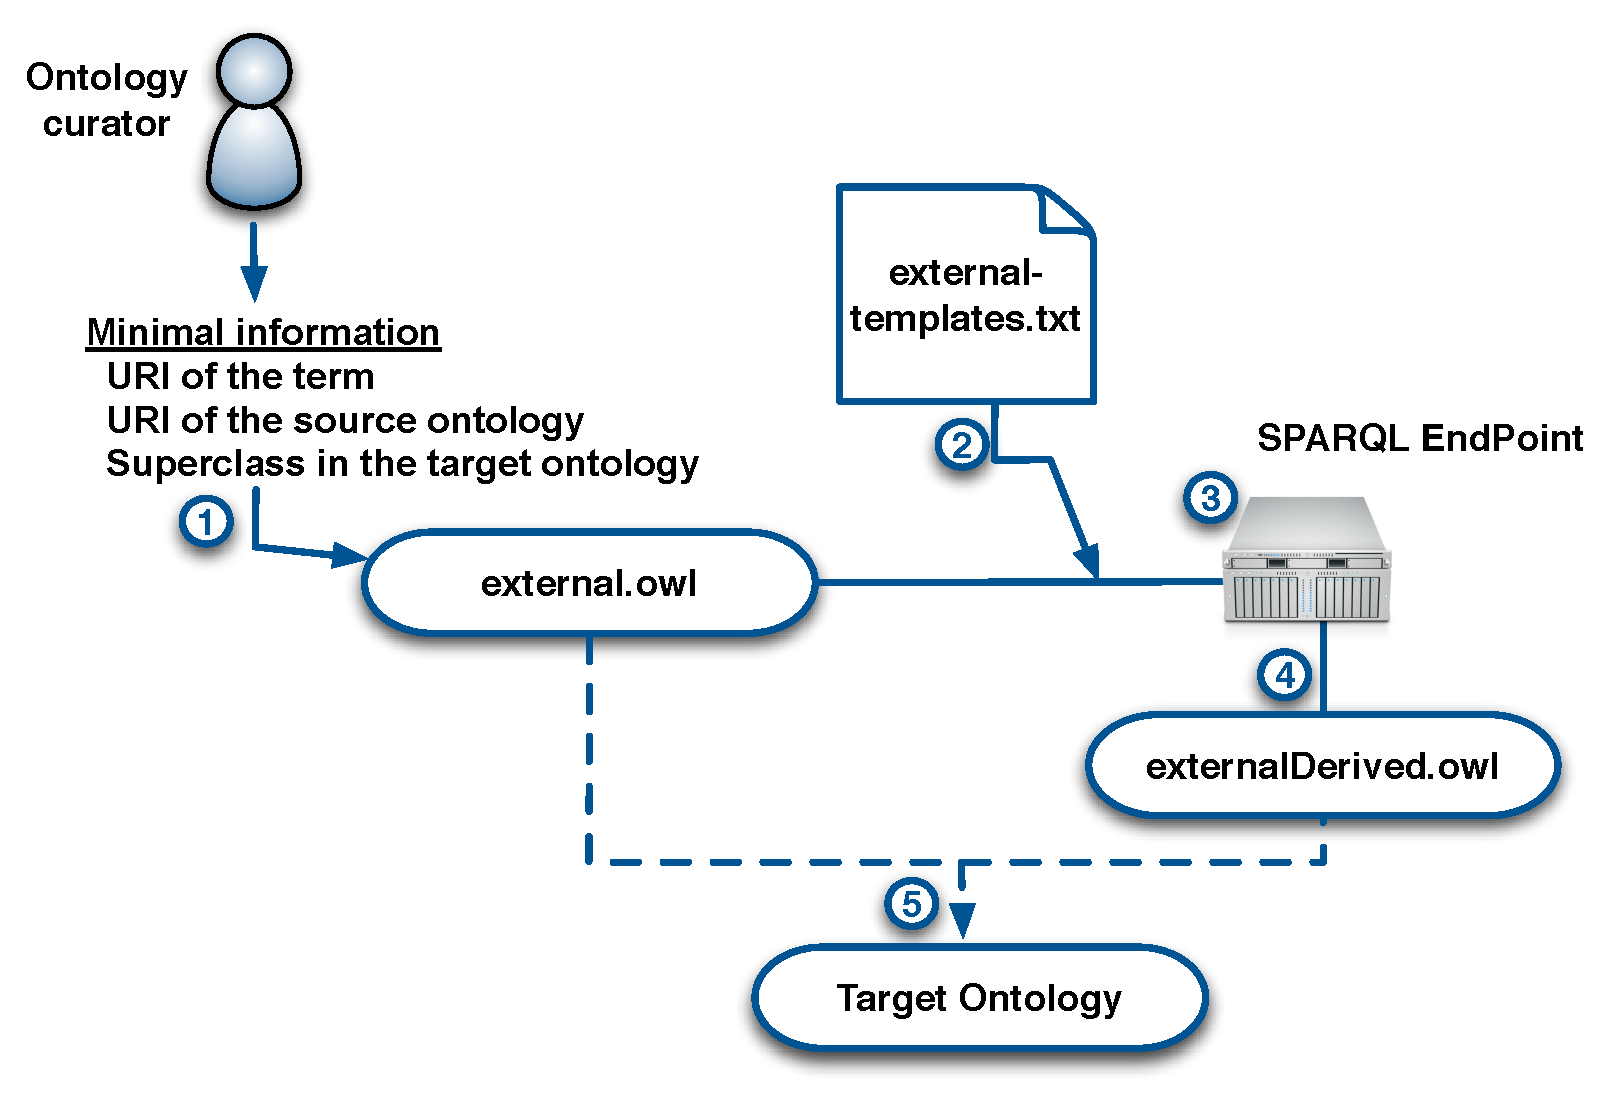
\includegraphics[width=.9\linewidth]{./figs/mechanism2.pdf}
}
\caption{Diagram of the MIREOT mechanism.
1. the minimal information is added into the external.owl file
2. a script parses the external.owl file, and for each class a sparql template is selected from external-templates.txt by matching the URI to patterns specified for each template. It uses the URI and the appropriate SPARQL template to generate a CONSTRUCT query
3. the SPARQL query is executed against a SPARQL endpoint (e.g. Neurocommons)
4. the results of the SPARQL queries are combined into the externalDerived.owl file
5. the target ontology imports the external.owl and externalDerived.owl files.
}
\label{fig:mechanism2}
\end{figure}



In the following sections we present two different cases of application of the \ac{MIREOT} guidelines, implemented during the \ac{OBI} development.


\subsection*{Use Case One - Basophil and Cell classes}

We replaced the \ac{OBI} class $Cell$ with that from the \ac{CL} ontology \cite{CL}. 
\ac{CL} is part of the \ac{OBO} Foundry effort, and we would like to use the $cell$ class as defined by this resource, instead of creating our own duplicated class.
This class can then be used in turn to import other classes as needed.
For example the following invocation of the \emph{add-to-external.pl} script:

\begin{footnotesize}
\begin{verbatim}
perl add-to-external.pl CL:0000767 CL:0000000 
\end{verbatim}
\end{footnotesize}

will add the class $basophil$ (CL:0000767) as subclass of the class $cell$  (CL:0000000), and set the source ontology URI as \url{http://purl.org/obo/owl/CL}.
Once imported, the $basophil$ and $cell$ classes can be used as would be any other OBI class. For example, the process $electroporation$ is defined as:

% Do you want to make this more formally manchester syntax? If so, no is_a and you need to add ``and'' where appropriate.
\begin{footnotesize}
\begin{verbatimtab}
is_a cell permeabilization
has_specified_input some cell
has_specified_output some 
   (cell and has_quality some electroporated))
utilizes_device some power supply
\end{verbatimtab}
\end{footnotesize}

More generally, additional axioms may be used to relate members of the class to other entities in the ontology.


\subsection*{Use Case Two - taxonomic information}

The \texttt{cell} use-case highlights what is likely to be the most common import scenario, \emph{i.e.}, a simple import of one external term, making it available for direct use in the target ontology.
However, in some cases, we may require more than that single external term, and to account for this \ac{MIREOT} has been devised to be flexible.

Consider the scenario in which we have two experiments, one in human and one in mouse. 
The files are annotated with the classes human and mouse from the ontology, which are in turn mapped from the NCBI taxonomy. 
We can easily imagine that somebody would want to have a query of the form ``give me all 
experiments in mammals''. In this case, we would need to know that human and mouse are 
subclasses (even indirect) of mammals in the NCBI taxonomy. Therefore, when mapping 
towards an NCBI term, we decided to retrieve all its superclasses as well up to the root of the 
NCBI taxonomy. As per the mechanism described above, the mapped class (\emph{e.g.}, human) is 
defined in external.owl, whereas this additional information to the human class (\emph{i.e.}, its 
superclasses) are stored in externalDerived.owl. 

When the \emph{create-external-derived.lisp} script parses the \emph{external.owl} file and encounters an NCBI taxonomy ID, it will therefore invoke a specific SPARQL query (cf figure \ref{fig:sparql2}). 

\begin{figure}[t]
\scriptsize
\verbatiminput{./figs/sparql2.txt} 
\caption{Template SPARQL query for import from the NCBI taxonomy. The \_ID\_GOES\_HERE\_ pattern will be replaced by the relevant NCBITax ID dynamically via script when building the CONSTRUCT query. This query allows retrieval of the class of interest and its parents up to a set of defined root classes. Note that the graph <http://purl.org/science/graph/obo/NCBITaxon> contains the source ontology, but the full store includes inferred subClassOf triples.}
\label{fig:sparql2}
\end{figure}
As per the mechanism described above, the minimum information about the imported external class (\emph{e.g.}, \emph{Mus musculus}) is defined in \emph{external.owl}, whereas the additional information (rank information - genus, kingdom, phylum, etc.) is stored in \emph{ externalDerived.owl}.


\section*{Discussion}

The \ac{MIREOT} mechanism is currently  implemented and used by several ontologies, including  \ac{OBI},  the \ac{IAO}\cite{IAO}, the \ac{VO}\cite{VO}, the \ac{IDO}\cite{IDO} and the \ac{InfluenzO}\cite{InfluenzO}.
In the context of \ac{OBI}, we currently explicitly import 472 terms, which in turn led to actual integration of 1447 classes (due to the automatic retrieval of parents when using the NCBI taxonomy). 

A consideration for using this approach is the status of assertions made on imported terms.
In adding axioms such as the subclass axiom when importing the external term, the aim is to only assert true statements, for instance those that the developers of the source ontology would agree with.
If such additional restrictions are required those should be stored in the importing ontology: the \emph{external.owl} and \emph{externalDerived.owl} are meant to include only the imported information.
We anticipate that some of the statements added by the importing ontology may migrate to the source ontologies at some point in the future; a fruit of the collaborative nature of OBO Foundry ontology development. 

If additional annotations are added to the imported terms (for example, we want to add an example of usage for the \ac{GO} imported term \textit{protein complex}), we also need to ensure that if the imported term is deprecated or replaced by an other (\emph{e.g.}, replacing  the \ac{GO} \textit{protein complex} term with the \ac{PRO} one), the annotation is similarly removed. 
With broader use of the MIREOT mechanism by OBI and other resources, several minor issues arose.

For example, consider the case of \ac{IAO} devlopers needing the term $investigation$.  This class already exists in \ac{OBI}, and \ac{IAO} developers therefore chose to \emph{MIREOT} it, effectively integrating the class \url{http://purl.obolibrary.org/obo/OBI_0000066} and distributing it as part of the \ac{IAO} releases.
However, \ac{OBI} imports \ac{IAO}, and therefore reimports, \emph{via IAO}, its own $investigation$ class. This is not problematic in general, redundancy of information in OWL files being of no consequence. However when \ac{OBI} curators decided to update the definition of the $investigation$ class, the information natively in \ac{OBI} and that imported from \ac{IAO} became out-of-sync: two different definitions were displayed to the curators. Moreover one of them couldn't be edited as it is not in the active ontology file.

One solution would be to update the \ac{IAO} import - but this requires a release of \ac{OBI} with the updated $investigation$ definition, its upload on Neurocommons, and for the \ac{IAO} developers to update their information and produce a new release of \ac{IAO}. At best, this implies a delay of a few days, more realistically of a few weeks until the information in both files is again synchronized.
Another solution that we think is more sensible would be for tools to recognize and prioritize the origin of a class based on its URI. Ontology editing tools would display only the information originating from the target ontology when editing the target ontology file.

Interestingly, this had an other consequence: when updating the information from Neurocommons, we needed to specify which \ac{RDF} graph \cite{RDF} the term \emph{originally} belongs to. Taking again our example of the $investigation$ class, when querying based on its URI without specifying the RDF graph, the SPARQL endpoint would return the \ac{OBI} class, but also the one distributed by \ac{IAO}, which is not the desired behavior: remember that in our example the \ac{IAO} annotation property values are now out of date compared to the original, authoritative \ac{OBI} file. As it turns out such examples of copying properties also occur where terms have been reused by different OBO ontologies.

This leads us to our last potential issue: when updating MIREOTed information (\emph{e.g.}, \ac{IAO} updates its \emph{externalDerived.owl} file), we need to ensure that the SPARQL endpoint where the information resides is up-to-date. As we currently rely on the \ac{OBO} Foundry resources, we know that the Neurocommons \ac{OBO} distribution is updated nightly with the latest information from the \ac{OBO} server, and we are therefore reasonably certain that we are working with current resources. This may not always be easy to know if extending the mechanism to an other SPARQL endpoint, or other sets of ontological resources.

When using the \ac{MIREOT} standard one must be cognizant of the trade-off between complete consistency checking and heavyweight importing versus lightweight importing but only partial consistency checking.
By copying only parts of an ontology there is the risk that inferences drawn may be incomplete or incorrect. 
Correct inference using the external classes is only guaranteed if the full ontologies, or a module, are imported.

Since we are doing only partial, reasoner supported, consistency checking, we take extra care when we need to make assertions about an imported term.
We review the textual definition and, if needed, talk with the original term editor to ensure we understand the denotation.
As we are importing from \ac{OBO} Foundry candidate ontologies we have a community process for monitoring change, a shared understanding of the basics of our domain, and the intention to eventually share the same upper-level ontology. 
Therefore, we expect that terms will be deprecated if there is a significant change in meaning, and are flexible enough to adjust and update our import of terms as the other ontologies start enhancing their logical definitions.


\section*{Future work}

The current implementation of the \ac{MIREOT} guidelines relies on command-line scripts, making it difficult for some curators to use. 
A webservice, OntoFox\cite{OntoFox}, has been developed by the He group at the University of Michigan to facilitate the process: ontology editors can use web forms to input their requirements, or submit specific OntoFox-formatted files for batch creation or update.
Ideally, a \protege\ \cite{Protege} plugin could be developed to improve the interaction between the curators and the tool and the implementation of the MIREOT guidelines. NCBO developers have created a widget allowing insertion of external references in an ontology\cite{NCBOWidget}, and we hope it will be updated to fully support the MIREOT guidelines.
In the future, we also expect to provide an option in the OBI distribution that replaces \emph{external.owl} with \emph{imports.owl}, a file of imports statements generated by extracting the ontology URIs mentioned in \emph{external.owl}.%\todo{include this in the diagram} MC: I don't see how to add this to the diagram
%Finally, we are also working on improving import of lower level terms under specific chosen root terms for 
As module extraction technology matures, we intend to include the ability to use such mechanisms for doing targeted imports, on a source by source basis.

%rewrite, moved to discussion: The MIREOT guidelines are currently being implemented by other ontologies, like the Vaccine Ontology (VO)\cite{VO}, and we ultimately hope that combined feedback will allow us to perfect the mechanism.

\section*{Acknowledgments}

In memory of our friend and colleague William Bug, Ontological Engineer. 

The OBI consortium is (in alphabetical order): Ryan Brinkman, Bill Bug, Helen Causton, Kevin Clancy, Christian Cocos, M\'elanie Courtot, Dirk Derom, Eric Deutsch, Liju Fan, Dawn Field, Jennifer Fostel, Gilberto Fragoso, Frank Gibson, Tanya Gray, Jason Greenbaum, Pierre Grenon, Jeff Grethe, Yongqun He, Mervi Heiskanen, Tina Hernandez-Boussard, Philip Lord, Allyson Lister, James Malone, Elisabetta Manduchi, Luisa Montecchi, Norman Morrison, Chris Mungall, Helen Parkinson, Bjoern Peters, Matthew Pocock, Philippe Rocca-Serra, Daniel Rubin, Alan Ruttenberg, Susanna-Assunta Sansone, Richard Scheuermann, Daniel Schober, Barry Smith, Larisa Soldatova, Holger Stenzhorn, Chris Stoeckert, Chris Taylor, John Westbrook,  Joe White, Trish Whetzel, Stefan Wiemann, Jie Zheng. 
The author's work is partially supported by funding from the NIH(R01EB005034),  the Public Health Agency of Canada / Canadian Institutes of Health Research Influenza Research Network (PCIRN), the EC EMERALD project (LSHG-CT-2006-037686), the BBSRC(BB/C008200/1, BB/D524283/1, BB/E025080/1), the EU FP7 DebugIT project (ICT-2007.5.2-217139), and the Michael Smith Foundation for Health Research.





\begin{thebibliography}{}


\bibitem{Grau}
Grau BC, Horrocks I, Kazakov Y, and Sattler U. (2007) . Extracting Modules from Ontologies: A Logic-based Approach. Proc. of the Third OWL Experiences and Directions Workshop, number 258 in CEUR 
\bibitem{Grau2}
 B. Cuenca Grau, I. Horrocks, Y. Kazakov and U. Sattler (2007) Just the right amount: Extracting modules from ontologies. In proc. of the 16th International World Wide Web Conference (WWW 2007) 
 \bibitem{Jimenez}
 E. Jimenez-Ruiz, B.Cuenca-Grau, U. Sattler, T. Schneider and R. Berlanga (2008) Safe and Economic Re-Use of Ontologies: A Logic-Based Methodology and Tool Support. 5th European Semantic Web Conference (ESWC 2008) 
 \bibitem{Seidenberg}
 J. Seidenberg, A. Rector (2006) Web ontology segmentation: analysis, classification and use. In proc. of the 15th International World Wide Web Conference (WWW 2006) 
 \bibitem{Sirin}
 Sirin, E., Parsia, B., Grau, B. C., Kalyanpur, A., and Katz, Y. (2007). Pellet: A practical OWL-DL reasoner. Web Semant. 5, 2 (Jun. 2007), 51-53. 
 
 
 
\bibitem{OWL} Web Ontology Language (OWL), \url{http://www.w3.org/2007/OWL/}.
\bibitem{NCBI} D. L. Wheeler, T. Barrett, D. A. Benson, S. H. Bryant, K. Canese, D. M. Church, M. DiCuccio, R. Edgar, S. Federhen, 
W. Helmberg, D. L. Kenton, O. Khovayko, D. J. Lipman, T. L. Madden, D. R. Maglott, J. Ostell, J. U. Pontius, K. D. Pruitt, 
G. D. Schuler, L. M. Schriml, E. Sequeira, S. T. Sherry, K. Sirotkin, G. Starchenko, T. O. Suzek, R. Tatusov, T. A. Tatusova, 
L. Wagner, and E. Yaschenko. Database resources of the national center for biotechnology information. Nucleic acids 
research, 33(Database issue):D39-45, Jan 1 2005.
\bibitem{FMA} C. Golbreich, S. Zhang, and O. Bodenreider. The foundational model of anatomy in owl: Experience and perspectives. Web 
semantics (Online), 4(3):181-195, 2006. 
\bibitem{OBI} OBI Ontology, \url{http://purl.obolibrary.org/obo/obi}.
\bibitem{BFO} P. Grenon, B. Smith, and L. Goldberg. Biodynamic ontology: applying bfo in the biomedical domain. Studies in health 
technology and informatics, 102:20-38, 2004. 
\bibitem{OBOFoundry} B. Smith, M. Ashburner, C. Rosse, J. Bard, W. Bug, W. Ceusters, L. J. Goldberg, K. Eilbeck, A. Ireland, C. J. Mungall, 
OBI Consortium, N. Leontis, P. Rocca-Serra, A. Ruttenberg, S. A. Sansone, R. H. Scheuermann, N. Shah, P. L. Whet- 
zel, and S. Lewis. The obo foundry: coordinated evolution of ontologies to support biomedical data integration. Nature 
biotechnology, 25(11):1251-1255, Nov 2007. 
\bibitem{CARO} Melissa A. Haendel, Fabian Neuhaus, David Osumi-Sutherland, Paula M. Mabee, Jose L.V. Mejino Jr., Chris J. Mungall, Barry Smith. CARO — The Common Anatomy Reference Ontology, in Anatomy Ontologies for Bioinformatics Principles and Practice, Series: Computational Biology , Vol. 6, ed. Burger, Albert; Davidson, Duncan; Baldock, Richard, 2008
\bibitem{GO} Gene Ontology Consortium. The gene ontology (go) database and informatics resource. Nucleic acids research, 
32(90001):D258-D261, 01/01/ 2004. 
\bibitem{GOGuide} Go editorial style guide - \url{http://www.geneontology.org/GO.usage.shtml}.
\bibitem{OBIScripts} OBI scripts -  \url{http://purl.obolibrary.org/obo/obi/repository/}.
\bibitem{SPARQL} SPARQL Query Language for RDF - \url{http://www.w3.org/TR/rdf- sparql- query/}. 
\bibitem{IAO} The Information Artifact Ontology (IAO), \url{http://code.google.com/p/information- artifact- ontology/}.
\bibitem{NeurocommonsSparql} Neurocommons OBO SPARQL endpoint - http://sparql.obo.neurocommons.org/. 
\bibitem{Neurocommons} Ruttenberg A, Rees J, Samwald M, Marshall M. Life sciences on the Semantic Web: the Neurocommons and beyond Briefings in Bioinformatics 10 , 193-204 2009 available at \url{http://purl.org/science/publication/neurocommons2009.pdf}
\bibitem{CL} J. Bard, S. Y. Rhee, and M. Ashburner. An ontology for cell types. Genome biology, 6(2):R21, 2005. 
\bibitem{VO} The Vaccine Ontology - \url{http://www.violinet.org/vaccineontology/}
\bibitem{Protege} The Prot\'{e}g\'{e} Ontology Editor and Knowledge Acquisition System, \url{http://protege.stanford.edu/}
\bibitem{IDO} The Infectious Disease Ontology - \url{http://www.infectiousdiseaseontology.org/}
\bibitem{InfluenzO} The Influenza Ontology - \url{https://sourceforge.net/projects/influenzo/}.
\bibitem{PRO} Darren A. Natale, Cecilia N. Arighi, Winona Barker, Judith Blake, Ti-Cheng Chang, Zhangzhi Hu, Hongfang Liu, Barry Smith, and Cathy H. Wu, "Framework for a Protein Ontology", Proceedings of the First International Workshop on Text Mining in Bioinformatics, 2006, pp. 29-36.
\bibitem{RDF} RDF/XML Syntax Specification - \url{http://www.w3.org/TR/rdf-syntax-grammar/}
\bibitem{PATO} Phenotypic Quality Ontology - \url{http://obofoundry.org/wiki/index.php/PATO:Main_Page}
\bibitem{ChEBI} Degtyarenko, K., de Matos, P., Ennis, M., Hastings, J., Zbinden, M., McNaught, A., Alcántara, R., Darsow, M., Guedj, M. and Ashburner, M. (2008) ChEBI: a database and ontology for chemical entities of biological interest. Nucleic Acids Res. 36, D344-D350.
\bibitem{NCBOWidget} BioPortal Reference Plugin - \url{http://protegewiki.stanford.edu/index.php/BioPortal_Reference_Plugin}.
\bibitem{OntoFox} OntoFox - \url{http://ontofox.hegroup.org/}.
\bibitem{OBIQueries} - SPARQL queries template file - \url{http://obi.svn.sourceforge.net/svnroot/obi/trunk/src/tools/build/external-templates.txt}

 
\end{thebibliography}
    
\begin{acronym}
\acro{BFO}{Basic Formal Ontology}

\acro{CL}{Cell Type}

\acro{GO}{Gene Ontology}

\acro{MIREOT}{Minimum Information to Reference an External Ontology Term}

\acro{OBI}{Ontology of Biomedical Investigations}
\acro{OBO}{Open Biomedical Ontologies}
\acro{OWL}{Web Ontology Language}
\acro{IAO}{Information Artifact Ontology}
\acro{VO}{Vaccine Ontology}
\acro{IDO}{Infectious Disease Ontology}
\acro{InfluenzO}{Influenza Ontology}
\acro{CARO}{Common Anatomy Reference Ontology}
\acro{PRO}{Protein Ontology}
\acro{RDF}{Resource Description Framework}
\acro{FMA}{Foundational Model of Anatomy}
\acro{PATO}{Phenotypic Quality Ontology}
\acro{ChEBI}{Chemical Entities of Biological Interest}

\end{acronym}




\end{document}
